\documentclass[1p]{elsarticle_modified}
%\bibliographystyle{elsarticle-num}

%\usepackage[colorlinks]{hyperref}
%\usepackage{abbrmath_seonhwa} %\Abb, \Ascr, \Acal ,\Abf, \Afrak
\usepackage{amsfonts}
\usepackage{amssymb}
\usepackage{amsmath}
\usepackage{amsthm}
\usepackage{scalefnt}
\usepackage{amsbsy}
\usepackage{kotex}
\usepackage{caption}
\usepackage{subfig}
\usepackage{color}
\usepackage{graphicx}
\usepackage{xcolor} %% white, black, red, green, blue, cyan, magenta, yellow
\usepackage{float}
\usepackage{setspace}
\usepackage{hyperref}

\usepackage{tikz}
\usetikzlibrary{arrows}

\usepackage{multirow}
\usepackage{array} % fixed length table
\usepackage{hhline}

%%%%%%%%%%%%%%%%%%%%%
\makeatletter
\renewcommand*\env@matrix[1][\arraystretch]{%
	\edef\arraystretch{#1}%
	\hskip -\arraycolsep
	\let\@ifnextchar\new@ifnextchar
	\array{*\c@MaxMatrixCols c}}
\makeatother %https://tex.stackexchange.com/questions/14071/how-can-i-increase-the-line-spacing-in-a-matrix
%%%%%%%%%%%%%%%

\usepackage[normalem]{ulem}

\newcommand{\msout}[1]{\ifmmode\text{\sout{\ensuremath{#1}}}\else\sout{#1}\fi}
%SOURCE: \msout is \stkout macro in https://tex.stackexchange.com/questions/20609/strikeout-in-math-mode

\newcommand{\cancel}[1]{
	\ifmmode
	{\color{red}\msout{#1}}
	\else
	{\color{red}\sout{#1}}
	\fi
}

\newcommand{\add}[1]{
	{\color{blue}\uwave{#1}}
}

\newcommand{\replace}[2]{
	\ifmmode
	{\color{red}\msout{#1}}{\color{blue}\uwave{#2}}
	\else
	{\color{red}\sout{#1}}{\color{blue}\uwave{#2}}
	\fi
}

\newcommand{\Sol}{\mathcal{S}} %segment
\newcommand{\D}{D} %diagram
\newcommand{\A}{\mathcal{A}} %arc


%%%%%%%%%%%%%%%%%%%%%%%%%%%%%5 test

\def\sl{\operatorname{\textup{SL}}(2,\Cbb)}
\def\psl{\operatorname{\textup{PSL}}(2,\Cbb)}
\def\quan{\mkern 1mu \triangleright \mkern 1mu}

\theoremstyle{definition}
\newtheorem{thm}{Theorem}[section]
\newtheorem{prop}[thm]{Proposition}
\newtheorem{lem}[thm]{Lemma}
\newtheorem{ques}[thm]{Question}
\newtheorem{cor}[thm]{Corollary}
\newtheorem{defn}[thm]{Definition}
\newtheorem{exam}[thm]{Example}
\newtheorem{rmk}[thm]{Remark}
\newtheorem{alg}[thm]{Algorithm}

\newcommand{\I}{\sqrt{-1}}
\begin{document}

%\begin{frontmatter}
%
%\title{Boundary parabolic representations of knots up to 8 crossings}
%
%%% Group authors per affiliation:
%\author{Yunhi Cho} 
%\address{Department of Mathematics, University of Seoul, Seoul, Korea}
%\ead{yhcho@uos.ac.kr}
%
%
%\author{Seonhwa Kim} %\fnref{s_kim}}
%\address{Center for Geometry and Physics, Institute for Basic Science, Pohang, 37673, Korea}
%\ead{ryeona17@ibs.re.kr}
%
%\author{Hyuk Kim}
%\address{Department of Mathematical Sciences, Seoul National University, Seoul 08826, Korea}
%\ead{hyukkim@snu.ac.kr}
%
%\author{Seokbeom Yoon}
%\address{Department of Mathematical Sciences, Seoul National University, Seoul, 08826,  Korea}
%\ead{sbyoon15@snu.ac.kr}
%
%\begin{abstract}
%We find all boundary parabolic representation of knots up to 8 crossings.
%
%\end{abstract}
%\begin{keyword}
%    \MSC[2010] 57M25 
%\end{keyword}
%
%\end{frontmatter}

%\linenumbers
%\tableofcontents
%
\newcommand\colored[1]{\textcolor{white}{\rule[-0.35ex]{0.8em}{1.4ex}}\kern-0.8em\color{red} #1}%
%\newcommand\colored[1]{\textcolor{white}{ #1}\kern-2.17ex	\textcolor{white}{ #1}\kern-1.81ex	\textcolor{white}{ #1}\kern-2.15ex\color{red}#1	}

{\Large $\underline{12a_{0147}~(K12a_{0147})}$}

\setlength{\tabcolsep}{10pt}
\renewcommand{\arraystretch}{1.6}
\vspace{1cm}\begin{tabular}{m{100pt}>{\centering\arraybackslash}m{274pt}}
\multirow{5}{120pt}{
	\centering
	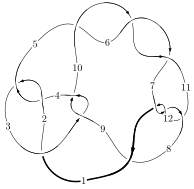
\includegraphics[width=112pt]{../../../GIT/diagram.site/Diagrams/png/948_12a_0147.png}\\
\ \ \ A knot diagram\footnotemark}&
\allowdisplaybreaks
\textbf{Linearized knot diagam} \\
\cline{2-2}
 &
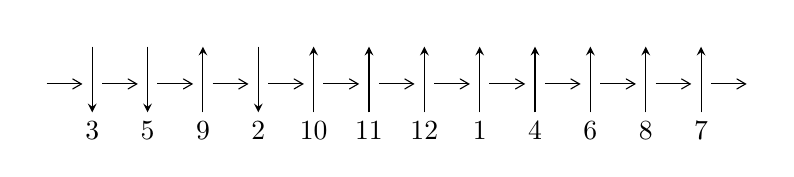
\begin{tikzpicture}[x=20pt, y=17pt]
	% nodes
	\node (C0) at (0, 0) {};
	\node (C1) at (1, 0) {};
	\node (C1U) at (1, +1) {};
	\node (C1D) at (1, -1) {3};

	\node (C2) at (2, 0) {};
	\node (C2U) at (2, +1) {};
	\node (C2D) at (2, -1) {5};

	\node (C3) at (3, 0) {};
	\node (C3U) at (3, +1) {};
	\node (C3D) at (3, -1) {9};

	\node (C4) at (4, 0) {};
	\node (C4U) at (4, +1) {};
	\node (C4D) at (4, -1) {2};

	\node (C5) at (5, 0) {};
	\node (C5U) at (5, +1) {};
	\node (C5D) at (5, -1) {10};

	\node (C6) at (6, 0) {};
	\node (C6U) at (6, +1) {};
	\node (C6D) at (6, -1) {11};

	\node (C7) at (7, 0) {};
	\node (C7U) at (7, +1) {};
	\node (C7D) at (7, -1) {12};

	\node (C8) at (8, 0) {};
	\node (C8U) at (8, +1) {};
	\node (C8D) at (8, -1) {1};

	\node (C9) at (9, 0) {};
	\node (C9U) at (9, +1) {};
	\node (C9D) at (9, -1) {4};

	\node (C10) at (10, 0) {};
	\node (C10U) at (10, +1) {};
	\node (C10D) at (10, -1) {6};

	\node (C11) at (11, 0) {};
	\node (C11U) at (11, +1) {};
	\node (C11D) at (11, -1) {8};

	\node (C12) at (12, 0) {};
	\node (C12U) at (12, +1) {};
	\node (C12D) at (12, -1) {7};
	\node (C13) at (13, 0) {};

	% arrows
	\draw[->,>={angle 60}]
	(C0) edge (C1) (C1) edge (C2) (C2) edge (C3) (C3) edge (C4) (C4) edge (C5) (C5) edge (C6) (C6) edge (C7) (C7) edge (C8) (C8) edge (C9) (C9) edge (C10) (C10) edge (C11) (C11) edge (C12) (C12) edge (C13) ;	\draw[->,>=stealth]
	(C1U) edge (C1D) (C2U) edge (C2D) (C3D) edge (C3U) (C4U) edge (C4D) (C5D) edge (C5U) (C6D) edge (C6U) (C7D) edge (C7U) (C8D) edge (C8U) (C9D) edge (C9U) (C10D) edge (C10U) (C11D) edge (C11U) (C12D) edge (C12U) ;
	\end{tikzpicture} \\
\hhline{~~} \\& 
\textbf{Solving Sequence} \\ \cline{2-2} 
 &
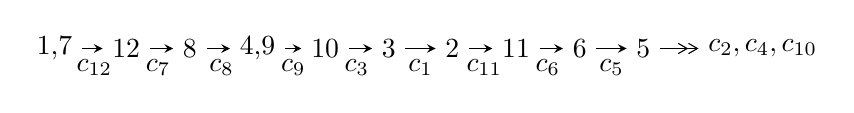
\begin{tikzpicture}[x=23pt, y=7pt]
	% node
	\node (A0) at (-1/8, 0) {1,7};
	\node (A1) at (1, 0) {12};
	\node (A2) at (2, 0) {8};
	\node (A3) at (49/16, 0) {4,9};
	\node (A4) at (33/8, 0) {10};
	\node (A5) at (41/8, 0) {3};
	\node (A6) at (49/8, 0) {2};
	\node (A7) at (57/8, 0) {11};
	\node (A8) at (65/8, 0) {6};
	\node (A9) at (73/8, 0) {5};
	\node (C1) at (1/2, -1) {$c_{12}$};
	\node (C2) at (3/2, -1) {$c_{7}$};
	\node (C3) at (5/2, -1) {$c_{8}$};
	\node (C4) at (29/8, -1) {$c_{9}$};
	\node (C5) at (37/8, -1) {$c_{3}$};
	\node (C6) at (45/8, -1) {$c_{1}$};
	\node (C7) at (53/8, -1) {$c_{11}$};
	\node (C8) at (61/8, -1) {$c_{6}$};
	\node (C9) at (69/8, -1) {$c_{5}$};
	\node (A10) at (11, 0) {$c_{2},c_{4},c_{10}$};

	% edge
	\draw[->,>=stealth]	
	(A0) edge (A1) (A1) edge (A2) (A2) edge (A3) (A3) edge (A4) (A4) edge (A5) (A5) edge (A6) (A6) edge (A7) (A7) edge (A8) (A8) edge (A9) ;
	\draw[->>,>={angle 60}]	
	(A9) edge (A10);
\end{tikzpicture} \\ 

\end{tabular} \\

\footnotetext{
The image of knot diagram is generated by the software ``\textbf{Draw programme}" developed by Andrew Bartholomew(\url{http://www.layer8.co.uk/maths/draw/index.htm\#Running-draw}), where we modified some parts for our purpose(\url{https://github.com/CATsTAILs/LinksPainter}).
}\phantom \\ \newline 
\centering \textbf{Ideals for irreducible components\footnotemark of $X_{\text{par}}$} 
 
\begin{align*}
I^u_{1}&=\langle 
u^{58}+u^{57}+\cdots+b- u,\;2 u^{57}- u^{56}+\cdots+a-1,\;u^{60}-2 u^{59}+\cdots-2 u+1\rangle \\
I^u_{2}&=\langle 
b-1,\;- u^4- u^3-2 u^2+a- u-1,\;u^6+u^5+3 u^4+2 u^3+2 u^2+u-1\rangle \\
\\
\end{align*}
\raggedright * 2 irreducible components of $\dim_{\mathbb{C}}=0$, with total 66 representations.\\
\footnotetext{All coefficients of polynomials are rational numbers. But the coefficients are sometimes approximated in decimal forms when there is not enough margin.}
\newpage
\renewcommand{\arraystretch}{1}
\centering \section*{I. $I^u_{1}= \langle u^{58}+u^{57}+\cdots+b- u,\;2 u^{57}- u^{56}+\cdots+a-1,\;u^{60}-2 u^{59}+\cdots-2 u+1 \rangle$}
\flushleft \textbf{(i) Arc colorings}\\
\begin{tabular}{m{7pt} m{180pt} m{7pt} m{180pt} }
\flushright $a_{1}=$&$\begin{pmatrix}1\\0\end{pmatrix}$ \\
\flushright $a_{7}=$&$\begin{pmatrix}0\\u\end{pmatrix}$ \\
\flushright $a_{12}=$&$\begin{pmatrix}1\\u^2\end{pmatrix}$ \\
\flushright $a_{8}=$&$\begin{pmatrix}u\\u^3+u\end{pmatrix}$ \\
\flushright $a_{4}=$&$\begin{pmatrix}-2 u^{57}+u^{56}+\cdots-5 u+1\\- u^{58}- u^{57}+\cdots+4 u^2+u\end{pmatrix}$ \\
\flushright $a_{9}=$&$\begin{pmatrix}u^3+2 u\\u^3+u\end{pmatrix}$ \\
\flushright $a_{10}=$&$\begin{pmatrix}- u^8-3 u^6-3 u^4+1\\- u^{10}-4 u^8-5 u^6+3 u^2\end{pmatrix}$ \\
\flushright $a_{3}=$&$\begin{pmatrix}- u^{55}+u^{54}+\cdots+13 u^2-5 u\\- u^{57}+u^{56}+\cdots-22 u^3+5 u^2\end{pmatrix}$ \\
\flushright $a_{2}=$&$\begin{pmatrix}u^{57}- u^{56}+\cdots-10 u^2+4 u\\u^{57}- u^{56}+\cdots+14 u^3-5 u^2\end{pmatrix}$ \\
\flushright $a_{11}=$&$\begin{pmatrix}u^2+1\\u^4+2 u^2\end{pmatrix}$ \\
\flushright $a_{6}=$&$\begin{pmatrix}- u^5-2 u^3- u\\- u^7-3 u^5-2 u^3+u\end{pmatrix}$ \\
\flushright $a_{5}=$&$\begin{pmatrix}u^{11}+4 u^9+6 u^7+2 u^5-3 u^3-2 u\\u^{13}+5 u^{11}+9 u^9+4 u^7-6 u^5-5 u^3+u\end{pmatrix}$\\&\end{tabular}
\flushleft \textbf{(ii) Obstruction class $= -1$}\\~\\
\flushleft \textbf{(iii) Cusp Shapes $= -4 u^{59}+8 u^{58}+\cdots+16 u+11$}\\~\\
\newpage\renewcommand{\arraystretch}{1}
\flushleft \textbf{(iv) u-Polynomials at the component}\newline \\
\begin{tabular}{m{50pt}|m{274pt}}
Crossings & \hspace{64pt}u-Polynomials at each crossing \\
\hline $$\begin{aligned}c_{1}\end{aligned}$$&$\begin{aligned}
&u^{60}+25 u^{59}+\cdots+71 u+1
\end{aligned}$\\
\hline $$\begin{aligned}c_{2},c_{4}\end{aligned}$$&$\begin{aligned}
&u^{60}-7 u^{59}+\cdots-15 u+1
\end{aligned}$\\
\hline $$\begin{aligned}c_{3},c_{9}\end{aligned}$$&$\begin{aligned}
&u^{60}- u^{59}+\cdots-128 u+64
\end{aligned}$\\
\hline $$\begin{aligned}c_{5},c_{6},c_{8}\\c_{10}\end{aligned}$$&$\begin{aligned}
&u^{60}+2 u^{59}+\cdots-22 u+17
\end{aligned}$\\
\hline $$\begin{aligned}c_{7},c_{11},c_{12}\end{aligned}$$&$\begin{aligned}
&u^{60}-2 u^{59}+\cdots-2 u+1
\end{aligned}$\\
\hline
\end{tabular}\\~\\
\newpage\renewcommand{\arraystretch}{1}
\flushleft \textbf{(v) Riley Polynomials at the component}\newline \\
\begin{tabular}{m{50pt}|m{274pt}}
Crossings & \hspace{64pt}Riley Polynomials at each crossing \\
\hline $$\begin{aligned}c_{1}\end{aligned}$$&$\begin{aligned}
&y^{60}+27 y^{59}+\cdots-5339 y+1
\end{aligned}$\\
\hline $$\begin{aligned}c_{2},c_{4}\end{aligned}$$&$\begin{aligned}
&y^{60}-25 y^{59}+\cdots-71 y+1
\end{aligned}$\\
\hline $$\begin{aligned}c_{3},c_{9}\end{aligned}$$&$\begin{aligned}
&y^{60}-39 y^{59}+\cdots-102400 y+4096
\end{aligned}$\\
\hline $$\begin{aligned}c_{5},c_{6},c_{8}\\c_{10}\end{aligned}$$&$\begin{aligned}
&y^{60}-74 y^{59}+\cdots-246 y+289
\end{aligned}$\\
\hline $$\begin{aligned}c_{7},c_{11},c_{12}\end{aligned}$$&$\begin{aligned}
&y^{60}+46 y^{59}+\cdots+2 y+1
\end{aligned}$\\
\hline
\end{tabular}\\~\\
\newpage\flushleft \textbf{(vi) Complex Volumes and Cusp Shapes}
$$\begin{array}{c|c|c}  
\text{Solutions to }I^u_{1}& \I (\text{vol} + \sqrt{-1}CS) & \text{Cusp shape}\\
 \hline 
\begin{aligned}
u &= -0.291512 + 1.030160 I \\
a &= -0.678030 - 1.056140 I \\
b &= -1.19725 + 0.90363 I\end{aligned}
 & \phantom{-}2.03627 + 3.48281 I & \phantom{-}9.26462 + 0. I\phantom{ +0.000000I} \\ \hline\begin{aligned}
u &= -0.291512 - 1.030160 I \\
a &= -0.678030 + 1.056140 I \\
b &= -1.19725 - 0.90363 I\end{aligned}
 & \phantom{-}2.03627 - 3.48281 I & \phantom{-}9.26462 + 0. I\phantom{ +0.000000I} \\ \hline\begin{aligned}
u &= \phantom{-}0.924382 + 0.020442 I \\
a &= \phantom{-}4.05935 - 0.66619 I \\
b &= \phantom{-}3.19998 - 0.28395 I\end{aligned}
 & \phantom{-}15.6684 + 2.9598 I & \phantom{-}14.3979 - 0.9035 I \\ \hline\begin{aligned}
u &= \phantom{-}0.924382 - 0.020442 I \\
a &= \phantom{-}4.05935 + 0.66619 I \\
b &= \phantom{-}3.19998 + 0.28395 I\end{aligned}
 & \phantom{-}15.6684 - 2.9598 I & \phantom{-}14.3979 + 0.9035 I \\ \hline\begin{aligned}
u &= \phantom{-}0.920041 + 0.033760 I \\
a &= -3.85415 + 1.05460 I \\
b &= -3.05121 + 0.44044 I\end{aligned}
 & \phantom{-}13.7623 + 9.2779 I & \phantom{-}12.25398 - 5.25271 I \\ \hline\begin{aligned}
u &= \phantom{-}0.920041 - 0.033760 I \\
a &= -3.85415 - 1.05460 I \\
b &= -3.05121 - 0.44044 I\end{aligned}
 & \phantom{-}13.7623 - 9.2779 I & \phantom{-}12.25398 + 5.25271 I \\ \hline\begin{aligned}
u &= -0.911537 + 0.010474 I \\
a &= \phantom{-}0.074147 + 0.576052 I \\
b &= \phantom{-}0.121976 + 0.842888 I\end{aligned}
 & \phantom{-}9.99754 - 2.62685 I & \phantom{-}11.37857 + 2.57042 I \\ \hline\begin{aligned}
u &= -0.911537 - 0.010474 I \\
a &= \phantom{-}0.074147 - 0.576052 I \\
b &= \phantom{-}0.121976 - 0.842888 I\end{aligned}
 & \phantom{-}9.99754 + 2.62685 I & \phantom{-}11.37857 - 2.57042 I \\ \hline\begin{aligned}
u &= \phantom{-}0.907065\phantom{ +0.000000I} \\
a &= -5.12768\phantom{ +0.000000I} \\
b &= -3.74684\phantom{ +0.000000I}\end{aligned}
 & \phantom{-}8.33706\phantom{ +0.000000I} & \phantom{-}11.8870\phantom{ +0.000000I} \\ \hline\begin{aligned}
u &= -0.858590\phantom{ +0.000000I} \\
a &= \phantom{-}0.363466\phantom{ +0.000000I} \\
b &= \phantom{-}0.491382\phantom{ +0.000000I}\end{aligned}
 & \phantom{-}6.74177\phantom{ +0.000000I} & \phantom{-}17.3790\phantom{ +0.000000I}\\
 \hline 
 \end{array}$$\newpage$$\begin{array}{c|c|c}  
\text{Solutions to }I^u_{1}& \I (\text{vol} + \sqrt{-1}CS) & \text{Cusp shape}\\
 \hline 
\begin{aligned}
u &= -0.312735 + 1.108170 I \\
a &= \phantom{-}0.561203 + 1.060260 I \\
b &= \phantom{-}1.21319 - 0.89450 I\end{aligned}
 & \phantom{-}3.00527 - 2.16368 I & \phantom{-0.000000 } 0 \\ \hline\begin{aligned}
u &= -0.312735 - 1.108170 I \\
a &= \phantom{-}0.561203 - 1.060260 I \\
b &= \phantom{-}1.21319 + 0.89450 I\end{aligned}
 & \phantom{-}3.00527 + 2.16368 I & \phantom{-0.000000 } 0 \\ \hline\begin{aligned}
u &= \phantom{-}0.220037 + 1.166580 I \\
a &= -0.541278 - 0.506954 I \\
b &= -0.442672 - 0.001765 I\end{aligned}
 & -2.04443 + 1.13435 I & \phantom{-0.000000 } 0 \\ \hline\begin{aligned}
u &= \phantom{-}0.220037 - 1.166580 I \\
a &= -0.541278 + 0.506954 I \\
b &= -0.442672 + 0.001765 I\end{aligned}
 & -2.04443 - 1.13435 I & \phantom{-0.000000 } 0 \\ \hline\begin{aligned}
u &= \phantom{-}0.090975 + 1.210730 I \\
a &= -0.625680 - 0.018522 I \\
b &= \phantom{-}0.008321 + 0.346144 I\end{aligned}
 & -2.94977 + 1.52826 I & \phantom{-0.000000 } 0 \\ \hline\begin{aligned}
u &= \phantom{-}0.090975 - 1.210730 I \\
a &= -0.625680 + 0.018522 I \\
b &= \phantom{-}0.008321 - 0.346144 I\end{aligned}
 & -2.94977 - 1.52826 I & \phantom{-0.000000 } 0 \\ \hline\begin{aligned}
u &= -0.216557 + 1.227250 I \\
a &= -0.06688 - 1.83452 I \\
b &= -1.97312 + 0.77412 I\end{aligned}
 & -3.87712 - 2.82894 I & \phantom{-0.000000 } 0 \\ \hline\begin{aligned}
u &= -0.216557 - 1.227250 I \\
a &= -0.06688 + 1.83452 I \\
b &= -1.97312 - 0.77412 I\end{aligned}
 & -3.87712 + 2.82894 I & \phantom{-0.000000 } 0 \\ \hline\begin{aligned}
u &= -0.023050 + 1.250010 I \\
a &= \phantom{-}1.380020 - 0.264318 I \\
b &= -0.591773 - 0.904308 I\end{aligned}
 & -5.85350 - 1.02296 I & \phantom{-0.000000 } 0 \\ \hline\begin{aligned}
u &= -0.023050 - 1.250010 I \\
a &= \phantom{-}1.380020 + 0.264318 I \\
b &= -0.591773 + 0.904308 I\end{aligned}
 & -5.85350 + 1.02296 I & \phantom{-0.000000 } 0\\
 \hline 
 \end{array}$$\newpage$$\begin{array}{c|c|c}  
\text{Solutions to }I^u_{1}& \I (\text{vol} + \sqrt{-1}CS) & \text{Cusp shape}\\
 \hline 
\begin{aligned}
u &= \phantom{-}0.245047 + 1.253190 I \\
a &= \phantom{-}0.378482 + 0.886324 I \\
b &= \phantom{-}0.132951 + 0.216928 I\end{aligned}
 & -2.88526 + 5.03495 I & \phantom{-0.000000 } 0 \\ \hline\begin{aligned}
u &= \phantom{-}0.245047 - 1.253190 I \\
a &= \phantom{-}0.378482 - 0.886324 I \\
b &= \phantom{-}0.132951 - 0.216928 I\end{aligned}
 & -2.88526 - 5.03495 I & \phantom{-0.000000 } 0 \\ \hline\begin{aligned}
u &= -0.705473 + 0.105742 I \\
a &= \phantom{-}1.36818 + 0.60284 I \\
b &= \phantom{-}1.53947 + 0.34903 I\end{aligned}
 & \phantom{-}5.97344 - 1.58067 I & \phantom{-}14.4844 + 1.7262 I \\ \hline\begin{aligned}
u &= -0.705473 - 0.105742 I \\
a &= \phantom{-}1.36818 - 0.60284 I \\
b &= \phantom{-}1.53947 - 0.34903 I\end{aligned}
 & \phantom{-}5.97344 + 1.58067 I & \phantom{-}14.4844 - 1.7262 I \\ \hline\begin{aligned}
u &= -0.683970 + 0.169452 I \\
a &= -1.37278 - 0.90433 I \\
b &= -1.63862 - 0.45396 I\end{aligned}
 & \phantom{-}4.53909 - 7.15924 I & \phantom{-}11.78808 + 7.26929 I \\ \hline\begin{aligned}
u &= -0.683970 - 0.169452 I \\
a &= -1.37278 + 0.90433 I \\
b &= -1.63862 + 0.45396 I\end{aligned}
 & \phantom{-}4.53909 + 7.15924 I & \phantom{-}11.78808 - 7.26929 I \\ \hline\begin{aligned}
u &= -0.289347 + 1.277000 I \\
a &= -0.288688 + 1.121530 I \\
b &= \phantom{-}1.51609 - 0.18929 I\end{aligned}
 & \phantom{-}1.70407 - 5.14058 I & \phantom{-0.000000 } 0 \\ \hline\begin{aligned}
u &= -0.289347 - 1.277000 I \\
a &= -0.288688 - 1.121530 I \\
b &= \phantom{-}1.51609 + 0.18929 I\end{aligned}
 & \phantom{-}1.70407 + 5.14058 I & \phantom{-0.000000 } 0 \\ \hline\begin{aligned}
u &= \phantom{-}0.132541 + 1.308630 I \\
a &= -0.406370 + 0.704082 I \\
b &= \phantom{-}0.249931 - 0.025514 I\end{aligned}
 & -3.38321 + 0.85618 I & \phantom{-0.000000 } 0 \\ \hline\begin{aligned}
u &= \phantom{-}0.132541 - 1.308630 I \\
a &= -0.406370 - 0.704082 I \\
b &= \phantom{-}0.249931 + 0.025514 I\end{aligned}
 & -3.38321 - 0.85618 I & \phantom{-0.000000 } 0\\
 \hline 
 \end{array}$$\newpage$$\begin{array}{c|c|c}  
\text{Solutions to }I^u_{1}& \I (\text{vol} + \sqrt{-1}CS) & \text{Cusp shape}\\
 \hline 
\begin{aligned}
u &= \phantom{-}0.066974 + 1.325380 I \\
a &= \phantom{-}0.781022 - 0.695467 I \\
b &= -0.543698 - 0.075581 I\end{aligned}
 & -4.16051 + 5.05095 I & \phantom{-0.000000 } 0 \\ \hline\begin{aligned}
u &= \phantom{-}0.066974 - 1.325380 I \\
a &= \phantom{-}0.781022 + 0.695467 I \\
b &= -0.543698 + 0.075581 I\end{aligned}
 & -4.16051 - 5.05095 I & \phantom{-0.000000 } 0 \\ \hline\begin{aligned}
u &= -0.396765 + 1.275800 I \\
a &= -0.075936 + 0.314839 I \\
b &= \phantom{-}0.490833 - 0.033606 I\end{aligned}
 & \phantom{-}2.77814 - 4.50220 I & \phantom{-0.000000 } 0 \\ \hline\begin{aligned}
u &= -0.396765 - 1.275800 I \\
a &= -0.075936 - 0.314839 I \\
b &= \phantom{-}0.490833 + 0.033606 I\end{aligned}
 & \phantom{-}2.77814 + 4.50220 I & \phantom{-0.000000 } 0 \\ \hline\begin{aligned}
u &= -0.266120 + 1.310510 I \\
a &= \phantom{-}0.553874 - 1.188430 I \\
b &= -1.70796 + 0.00761 I\end{aligned}
 & -0.07047 - 10.54190 I & \phantom{-0.000000 } 0 \\ \hline\begin{aligned}
u &= -0.266120 - 1.310510 I \\
a &= \phantom{-}0.553874 + 1.188430 I \\
b &= -1.70796 - 0.00761 I\end{aligned}
 & -0.07047 + 10.54190 I & \phantom{-0.000000 } 0 \\ \hline\begin{aligned}
u &= \phantom{-}0.457433 + 1.260060 I \\
a &= -1.82540 + 1.52099 I \\
b &= -2.98099 - 0.61431 I\end{aligned}
 & \phantom{-}9.96888 - 4.36737 I & \phantom{-0.000000 } 0 \\ \hline\begin{aligned}
u &= \phantom{-}0.457433 - 1.260060 I \\
a &= -1.82540 - 1.52099 I \\
b &= -2.98099 + 0.61431 I\end{aligned}
 & \phantom{-}9.96888 + 4.36737 I & \phantom{-0.000000 } 0 \\ \hline\begin{aligned}
u &= -0.442079 + 1.277110 I \\
a &= \phantom{-}0.504030 + 0.136393 I \\
b &= -0.009416 - 0.838158 I\end{aligned}
 & \phantom{-}6.06778 - 2.20599 I & \phantom{-0.000000 } 0 \\ \hline\begin{aligned}
u &= -0.442079 - 1.277110 I \\
a &= \phantom{-}0.504030 - 0.136393 I \\
b &= -0.009416 + 0.838158 I\end{aligned}
 & \phantom{-}6.06778 + 2.20599 I & \phantom{-0.000000 } 0\\
 \hline 
 \end{array}$$\newpage$$\begin{array}{c|c|c}  
\text{Solutions to }I^u_{1}& \I (\text{vol} + \sqrt{-1}CS) & \text{Cusp shape}\\
 \hline 
\begin{aligned}
u &= \phantom{-}0.456253 + 1.272990 I \\
a &= \phantom{-}1.76917 - 1.83592 I \\
b &= \phantom{-}3.14034 + 0.47569 I\end{aligned}
 & \phantom{-}11.78740 + 1.96281 I & \phantom{-0.000000 } 0 \\ \hline\begin{aligned}
u &= \phantom{-}0.456253 - 1.272990 I \\
a &= \phantom{-}1.76917 + 1.83592 I \\
b &= \phantom{-}3.14034 - 0.47569 I\end{aligned}
 & \phantom{-}11.78740 - 1.96281 I & \phantom{-0.000000 } 0 \\ \hline\begin{aligned}
u &= \phantom{-}0.435543 + 1.284440 I \\
a &= -2.03302 + 2.66752 I \\
b &= -3.71170 - 0.21616 I\end{aligned}
 & \phantom{-}4.34700 + 4.79676 I & \phantom{-0.000000 } 0 \\ \hline\begin{aligned}
u &= \phantom{-}0.435543 - 1.284440 I \\
a &= -2.03302 - 2.66752 I \\
b &= -3.71170 + 0.21616 I\end{aligned}
 & \phantom{-}4.34700 - 4.79676 I & \phantom{-0.000000 } 0 \\ \hline\begin{aligned}
u &= -0.436271 + 1.293570 I \\
a &= -0.519420 - 0.001879 I \\
b &= \phantom{-}0.243847 + 0.801514 I\end{aligned}
 & \phantom{-}5.94185 - 7.44193 I & \phantom{-0.000000 } 0 \\ \hline\begin{aligned}
u &= -0.436271 - 1.293570 I \\
a &= -0.519420 + 0.001879 I \\
b &= \phantom{-}0.243847 - 0.801514 I\end{aligned}
 & \phantom{-}5.94185 + 7.44193 I & \phantom{-0.000000 } 0 \\ \hline\begin{aligned}
u &= \phantom{-}0.442698 + 1.304280 I \\
a &= \phantom{-}1.24864 - 2.54832 I \\
b &= \phantom{-}3.18374 - 0.09677 I\end{aligned}
 & \phantom{-}11.54400 + 7.84056 I & \phantom{-0.000000 } 0 \\ \hline\begin{aligned}
u &= \phantom{-}0.442698 - 1.304280 I \\
a &= \phantom{-}1.24864 + 2.54832 I \\
b &= \phantom{-}3.18374 + 0.09677 I\end{aligned}
 & \phantom{-}11.54400 - 7.84056 I & \phantom{-0.000000 } 0 \\ \hline\begin{aligned}
u &= \phantom{-}0.616209 + 0.070001 I \\
a &= -0.315993 + 1.163010 I \\
b &= -0.151276 + 0.030346 I\end{aligned}
 & \phantom{-}1.15428 + 1.92974 I & \phantom{-}10.88557 - 4.32279 I \\ \hline\begin{aligned}
u &= \phantom{-}0.616209 - 0.070001 I \\
a &= -0.315993 - 1.163010 I \\
b &= -0.151276 - 0.030346 I\end{aligned}
 & \phantom{-}1.15428 - 1.92974 I & \phantom{-}10.88557 + 4.32279 I\\
 \hline 
 \end{array}$$\newpage$$\begin{array}{c|c|c}  
\text{Solutions to }I^u_{1}& \I (\text{vol} + \sqrt{-1}CS) & \text{Cusp shape}\\
 \hline 
\begin{aligned}
u &= \phantom{-}0.435774 + 1.312250 I \\
a &= -1.01023 + 2.65881 I \\
b &= -3.05202 + 0.27246 I\end{aligned}
 & \phantom{-}9.5655 + 14.1217 I & \phantom{-0.000000 } 0 \\ \hline\begin{aligned}
u &= \phantom{-}0.435774 - 1.312250 I \\
a &= -1.01023 - 2.65881 I \\
b &= -3.05202 - 0.27246 I\end{aligned}
 & \phantom{-}9.5655 - 14.1217 I & \phantom{-0.000000 } 0 \\ \hline\begin{aligned}
u &= \phantom{-}0.329295 + 0.475961 I \\
a &= \phantom{-}0.395337 - 0.738913 I \\
b &= -0.440113 + 0.509380 I\end{aligned}
 & \phantom{-}1.24419 + 3.93574 I & \phantom{-}8.26947 - 6.96230 I \\ \hline\begin{aligned}
u &= \phantom{-}0.329295 - 0.475961 I \\
a &= \phantom{-}0.395337 + 0.738913 I \\
b &= -0.440113 - 0.509380 I\end{aligned}
 & \phantom{-}1.24419 - 3.93574 I & \phantom{-}8.26947 + 6.96230 I \\ \hline\begin{aligned}
u &= -0.566627\phantom{ +0.000000I} \\
a &= -2.54741\phantom{ +0.000000I} \\
b &= -2.01582\phantom{ +0.000000I}\end{aligned}
 & -0.173331\phantom{ +0.000000I} & \phantom{-}14.7800\phantom{ +0.000000I} \\ \hline\begin{aligned}
u &= \phantom{-}0.421793 + 0.356280 I \\
a &= -0.581552 + 0.715018 I \\
b &= \phantom{-}0.190880 - 0.469674 I\end{aligned}
 & \phantom{-}1.63592 - 0.97554 I & \phantom{-}10.14221 - 1.13061 I \\ \hline\begin{aligned}
u &= \phantom{-}0.421793 - 0.356280 I \\
a &= -0.581552 - 0.715018 I \\
b &= \phantom{-}0.190880 + 0.469674 I\end{aligned}
 & \phantom{-}1.63592 + 0.97554 I & \phantom{-}10.14221 + 1.13061 I \\ \hline\begin{aligned}
u &= \phantom{-}0.342205\phantom{ +0.000000I} \\
a &= -0.672021\phantom{ +0.000000I} \\
b &= \phantom{-}0.116519\phantom{ +0.000000I}\end{aligned}
 & \phantom{-}0.576782\phantom{ +0.000000I} & \phantom{-}17.2090\phantom{ +0.000000I} \\ \hline\begin{aligned}
u &= -0.131606 + 0.232247 I \\
a &= \phantom{-}0.11377 - 2.33220 I \\
b &= -0.662340 - 0.292492 I\end{aligned}
 & -1.60725 - 0.57664 I & -2.01562 + 2.57957 I \\ \hline\begin{aligned}
u &= -0.131606 - 0.232247 I \\
a &= \phantom{-}0.11377 + 2.33220 I \\
b &= -0.662340 + 0.292492 I\end{aligned}
 & -1.60725 + 0.57664 I & -2.01562 - 2.57957 I\\
 \hline 
 \end{array}$$\newpage\newpage\renewcommand{\arraystretch}{1}
\centering \section*{II. $I^u_{2}= \langle b-1,\;- u^4- u^3-2 u^2+a- u-1,\;u^6+u^5+3 u^4+2 u^3+2 u^2+u-1 \rangle$}
\flushleft \textbf{(i) Arc colorings}\\
\begin{tabular}{m{7pt} m{180pt} m{7pt} m{180pt} }
\flushright $a_{1}=$&$\begin{pmatrix}1\\0\end{pmatrix}$ \\
\flushright $a_{7}=$&$\begin{pmatrix}0\\u\end{pmatrix}$ \\
\flushright $a_{12}=$&$\begin{pmatrix}1\\u^2\end{pmatrix}$ \\
\flushright $a_{8}=$&$\begin{pmatrix}u\\u^3+u\end{pmatrix}$ \\
\flushright $a_{4}=$&$\begin{pmatrix}u^4+u^3+2 u^2+u+1\\1\end{pmatrix}$ \\
\flushright $a_{9}=$&$\begin{pmatrix}u^3+2 u\\u^3+u\end{pmatrix}$ \\
\flushright $a_{10}=$&$\begin{pmatrix}u^3+2 u\\u^3+u\end{pmatrix}$ \\
\flushright $a_{3}=$&$\begin{pmatrix}u^4+u^3+2 u^2+u+1\\1\end{pmatrix}$ \\
\flushright $a_{2}=$&$\begin{pmatrix}u^4+u^3+2 u^2+u+2\\1\end{pmatrix}$ \\
\flushright $a_{11}=$&$\begin{pmatrix}u^2+1\\u^4+2 u^2\end{pmatrix}$ \\
\flushright $a_{6}=$&$\begin{pmatrix}- u^5-2 u^3- u\\- u^5- u^4-2 u^3- u^2- u+1\end{pmatrix}$ \\
\flushright $a_{5}=$&$\begin{pmatrix}-1\\0\end{pmatrix}$\\&\end{tabular}
\flushleft \textbf{(ii) Obstruction class $= 1$}\\~\\
\flushleft \textbf{(iii) Cusp Shapes $= 3 u^4+2 u^3+5 u^2+2 u+3$}\\~\\
\newpage\renewcommand{\arraystretch}{1}
\flushleft \textbf{(iv) u-Polynomials at the component}\newline \\
\begin{tabular}{m{50pt}|m{274pt}}
Crossings & \hspace{64pt}u-Polynomials at each crossing \\
\hline $$\begin{aligned}c_{1},c_{2}\end{aligned}$$&$\begin{aligned}
&(u-1)^6
\end{aligned}$\\
\hline $$\begin{aligned}c_{3},c_{9}\end{aligned}$$&$\begin{aligned}
&u^6
\end{aligned}$\\
\hline $$\begin{aligned}c_{4}\end{aligned}$$&$\begin{aligned}
&(u+1)^6
\end{aligned}$\\
\hline $$\begin{aligned}c_{5},c_{6},c_{8}\end{aligned}$$&$\begin{aligned}
&u^6+u^5-3 u^4-2 u^3+2 u^2- u-1
\end{aligned}$\\
\hline $$\begin{aligned}c_{7}\end{aligned}$$&$\begin{aligned}
&u^6- u^5+3 u^4-2 u^3+2 u^2- u-1
\end{aligned}$\\
\hline $$\begin{aligned}c_{10}\end{aligned}$$&$\begin{aligned}
&u^6- u^5-3 u^4+2 u^3+2 u^2+u-1
\end{aligned}$\\
\hline $$\begin{aligned}c_{11},c_{12}\end{aligned}$$&$\begin{aligned}
&u^6+u^5+3 u^4+2 u^3+2 u^2+u-1
\end{aligned}$\\
\hline
\end{tabular}\\~\\
\newpage\renewcommand{\arraystretch}{1}
\flushleft \textbf{(v) Riley Polynomials at the component}\newline \\
\begin{tabular}{m{50pt}|m{274pt}}
Crossings & \hspace{64pt}Riley Polynomials at each crossing \\
\hline $$\begin{aligned}c_{1},c_{2},c_{4}\end{aligned}$$&$\begin{aligned}
&(y-1)^6
\end{aligned}$\\
\hline $$\begin{aligned}c_{3},c_{9}\end{aligned}$$&$\begin{aligned}
&y^6
\end{aligned}$\\
\hline $$\begin{aligned}c_{5},c_{6},c_{8}\\c_{10}\end{aligned}$$&$\begin{aligned}
&y^6-7 y^5+17 y^4-16 y^3+6 y^2-5 y+1
\end{aligned}$\\
\hline $$\begin{aligned}c_{7},c_{11},c_{12}\end{aligned}$$&$\begin{aligned}
&y^6+5 y^5+9 y^4+4 y^3-6 y^2-5 y+1
\end{aligned}$\\
\hline
\end{tabular}\\~\\
\newpage\flushleft \textbf{(vi) Complex Volumes and Cusp Shapes}
$$\begin{array}{c|c|c}  
\text{Solutions to }I^u_{2}& \I (\text{vol} + \sqrt{-1}CS) & \text{Cusp shape}\\
 \hline 
\begin{aligned}
u &= -0.873214\phantom{ +0.000000I} \\
a &= \phantom{-}1.56737\phantom{ +0.000000I} \\
b &= \phantom{-}1.00000\phantom{ +0.000000I}\end{aligned}
 & \phantom{-}6.01515\phantom{ +0.000000I} & \phantom{-}5.47870\phantom{ +0.000000I} \\ \hline\begin{aligned}
u &= \phantom{-}0.138835 + 1.234450 I \\
a &= -0.356069 - 0.921195 I \\
b &= \phantom{-}1.00000\phantom{ +0.000000I}\end{aligned}
 & -4.60518 + 1.97241 I & \phantom{-}0.92955 - 2.53106 I \\ \hline\begin{aligned}
u &= \phantom{-}0.138835 - 1.234450 I \\
a &= -0.356069 + 0.921195 I \\
b &= \phantom{-}1.00000\phantom{ +0.000000I}\end{aligned}
 & -4.60518 - 1.97241 I & \phantom{-}0.92955 + 2.53106 I \\ \hline\begin{aligned}
u &= -0.408802 + 1.276380 I \\
a &= \phantom{-}0.645284 + 0.801205 I \\
b &= \phantom{-}1.00000\phantom{ +0.000000I}\end{aligned}
 & \phantom{-}2.05064 - 4.59213 I & \phantom{-}1.87701 + 3.61028 I \\ \hline\begin{aligned}
u &= -0.408802 - 1.276380 I \\
a &= \phantom{-}0.645284 - 0.801205 I \\
b &= \phantom{-}1.00000\phantom{ +0.000000I}\end{aligned}
 & \phantom{-}2.05064 + 4.59213 I & \phantom{-}1.87701 - 3.61028 I \\ \hline\begin{aligned}
u &= \phantom{-}0.413150\phantom{ +0.000000I} \\
a &= \phantom{-}1.85419\phantom{ +0.000000I} \\
b &= \phantom{-}1.00000\phantom{ +0.000000I}\end{aligned}
 & -0.906083\phantom{ +0.000000I} & \phantom{-}4.90820\phantom{ +0.000000I}\\
 \hline 
 \end{array}$$\newpage
\newpage\renewcommand{\arraystretch}{1}
\centering \section*{ III. u-Polynomials}
\begin{tabular}{m{50pt}|m{274pt}}
Crossings & \hspace{64pt}u-Polynomials at each crossing \\
\hline $$\begin{aligned}c_{1}\end{aligned}$$&$\begin{aligned}
&((u-1)^6)(u^{60}+25 u^{59}+\cdots+71 u+1)
\end{aligned}$\\
\hline $$\begin{aligned}c_{2}\end{aligned}$$&$\begin{aligned}
&((u-1)^6)(u^{60}-7 u^{59}+\cdots-15 u+1)
\end{aligned}$\\
\hline $$\begin{aligned}c_{3},c_{9}\end{aligned}$$&$\begin{aligned}
&u^6(u^{60}- u^{59}+\cdots-128 u+64)
\end{aligned}$\\
\hline $$\begin{aligned}c_{4}\end{aligned}$$&$\begin{aligned}
&((u+1)^6)(u^{60}-7 u^{59}+\cdots-15 u+1)
\end{aligned}$\\
\hline $$\begin{aligned}c_{5},c_{6},c_{8}\end{aligned}$$&$\begin{aligned}
&(u^6+u^5-3 u^4-2 u^3+2 u^2- u-1)(u^{60}+2 u^{59}+\cdots-22 u+17)
\end{aligned}$\\
\hline $$\begin{aligned}c_{7}\end{aligned}$$&$\begin{aligned}
&(u^6- u^5+3 u^4-2 u^3+2 u^2- u-1)(u^{60}-2 u^{59}+\cdots-2 u+1)
\end{aligned}$\\
\hline $$\begin{aligned}c_{10}\end{aligned}$$&$\begin{aligned}
&(u^6- u^5-3 u^4+2 u^3+2 u^2+u-1)(u^{60}+2 u^{59}+\cdots-22 u+17)
\end{aligned}$\\
\hline $$\begin{aligned}c_{11},c_{12}\end{aligned}$$&$\begin{aligned}
&(u^6+u^5+3 u^4+2 u^3+2 u^2+u-1)(u^{60}-2 u^{59}+\cdots-2 u+1)
\end{aligned}$\\
\hline
\end{tabular}\newpage\renewcommand{\arraystretch}{1}
\centering \section*{ IV. Riley Polynomials}
\begin{tabular}{m{50pt}|m{274pt}}
Crossings & \hspace{64pt}Riley Polynomials at each crossing \\
\hline $$\begin{aligned}c_{1}\end{aligned}$$&$\begin{aligned}
&((y-1)^6)(y^{60}+27 y^{59}+\cdots-5339 y+1)
\end{aligned}$\\
\hline $$\begin{aligned}c_{2},c_{4}\end{aligned}$$&$\begin{aligned}
&((y-1)^6)(y^{60}-25 y^{59}+\cdots-71 y+1)
\end{aligned}$\\
\hline $$\begin{aligned}c_{3},c_{9}\end{aligned}$$&$\begin{aligned}
&y^6(y^{60}-39 y^{59}+\cdots-102400 y+4096)
\end{aligned}$\\
\hline $$\begin{aligned}c_{5},c_{6},c_{8}\\c_{10}\end{aligned}$$&$\begin{aligned}
&(y^6-7 y^5+17 y^4-16 y^3+6 y^2-5 y+1)\\
&\cdot(y^{60}-74 y^{59}+\cdots-246 y+289)
\end{aligned}$\\
\hline $$\begin{aligned}c_{7},c_{11},c_{12}\end{aligned}$$&$\begin{aligned}
&(y^6+5 y^5+\cdots-5 y+1)(y^{60}+46 y^{59}+\cdots+2 y+1)
\end{aligned}$\\
\hline
\end{tabular}
\vskip 2pc
\end{document}